\documentclass[11pt,letterpaper]{article}

\addtolength{\oddsidemargin}{-.875in}
\addtolength{\evensidemargin}{-.875in}
\addtolength{\textwidth}{1.75in}

\addtolength{\topmargin}{-.875in}
\addtolength{\textheight}{1.75in}

\usepackage[utf8]{inputenc}
\usepackage{caption} % for table captions
\usepackage{amsmath} % for multi-line equations and piecewises
\DeclareMathOperator{\sign}{sign}
\usepackage{graphicx}
\usepackage{relsize}
\usepackage{xspace}
\usepackage{verbatim} % for block comments
\usepackage{subcaption} % for subfigures
\usepackage{enumitem} % for a) b) c) lists
\newcommand{\Cyclus}{\textsc{Cyclus}\xspace}%
\newcommand{\Cycamore}{\textsc{Cycamore}\xspace}%
\newcommand{\deploy}{\texttt{d3ploy}\xspace}%
\newcommand{\Deploy}{\texttt{D3ploy}\xspace}%
\usepackage{tabularx}
\usepackage{color}
\usepackage{multirow}
\usepackage{float} 
\usepackage[acronym,toc]{glossaries}
%\include{acros}
\definecolor{bg}{rgb}{0.95,0.95,0.95}
\newcolumntype{b}{X}
\newcolumntype{f}{>{\hsize=.15\hsize}X}
\newcolumntype{s}{>{\hsize=.5\hsize}X}
\newcolumntype{m}{>{\hsize=.75\hsize}X}
\newcolumntype{r}{>{\hsize=1.1\hsize}X}
\usepackage{titling}
\usepackage[hang,flushmargin]{footmisc}
\renewcommand*\footnoterule{}
\usepackage{tikz}

\usetikzlibrary{shapes.geometric,arrows}
\tikzstyle{process} = [rectangle, rounded corners, 
minimum width=1cm, minimum height=1cm,text centered, draw=black, 
fill=blue!30]
\tikzstyle{arrow} = [thick,->,>=stealth]

\graphicspath{}

\begin{document}

\section{Advection}

	\subsection{advec1-t}

	\begin{itemize}
		\item \textit{advec1-t.i}
		\item 1D generated mesh with libmesh
		\item Uses DG Kernels
		\item InflowBC and OutflowBC
		\item Transient problem
	\end{itemize}

    Figure \ref{fig:advec1-t} shows the results.
    Advects BC.
    It seems like the variable has to be a CONSTANT MONOMIAL.

	\begin{equation}
    \frac{\partial}{\partial t}\rho + v \frac{\partial}{\partial x} \rho = 0
	\end{equation}

	\begin{figure}[htbp!]
		\centering
		\begin{subfigure}[t]{0.4\textwidth}
			\centering
			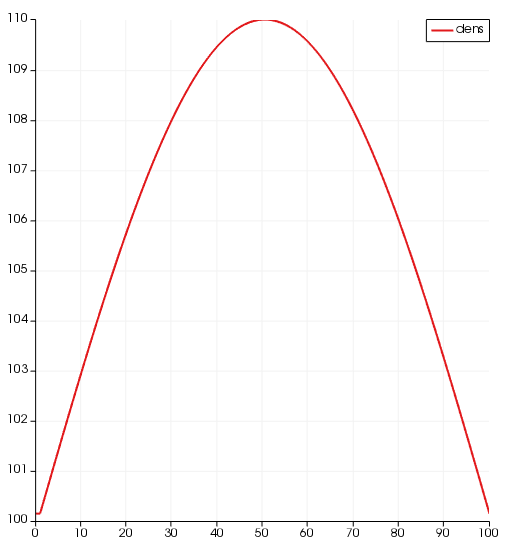
\includegraphics[width=\linewidth]{advec1-tA}
			\caption{t=0.}
		\end{subfigure}
		\begin{subfigure}[t]{0.4\textwidth}
			\centering
			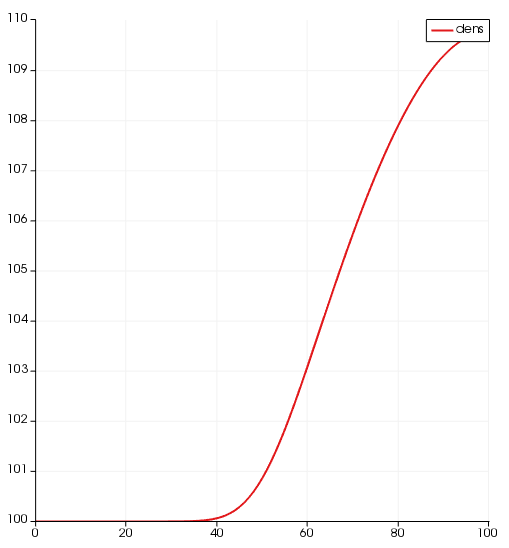
\includegraphics[width=\linewidth]{advec1-tB}
			\caption{t=100.}
		\end{subfigure}
		\hfill
		\caption{Advected density.}
		\label{fig:advec1-t}
	\end{figure}

    \subsection{periodic\_bc2}

	\begin{itemize}
		\item \textit{moose/examples/ex04\_bcs/periodic\_bc2.i}
		\item 1D generated mesh with libmesh
		\item Periodic BCs
		\item Transient problem
	\end{itemize}

    In \textit{advec1-t-bc.i} I tried to add periodicBCs to the previous problem and it does not work.
    Here I tried to isolate the problem.
    Figure \ref{fig:periodic} shows the results.
    It does not work if the valiable is a CONSTANT MONOMIAL.
    It works if the variable is FIRST order (either MONOMIAL or LAGRANGE).

	\begin{figure}[htbp!]
		\centering
		\begin{subfigure}[t]{0.4\textwidth}
			\centering
			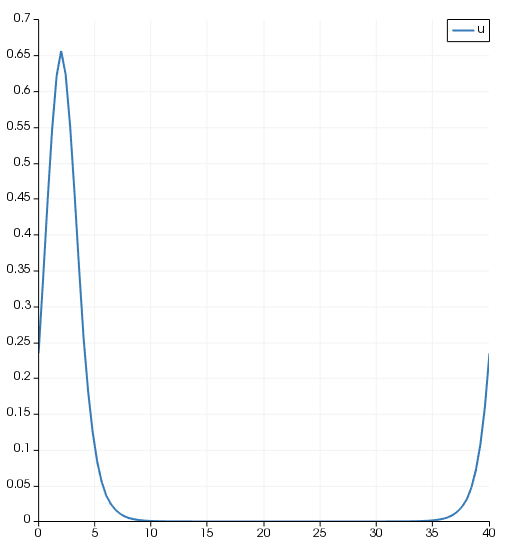
\includegraphics[width=\linewidth]{periodic_bc2_1}
			\caption{t=0.}
		\end{subfigure}
		\begin{subfigure}[t]{0.4\textwidth}
			\centering
			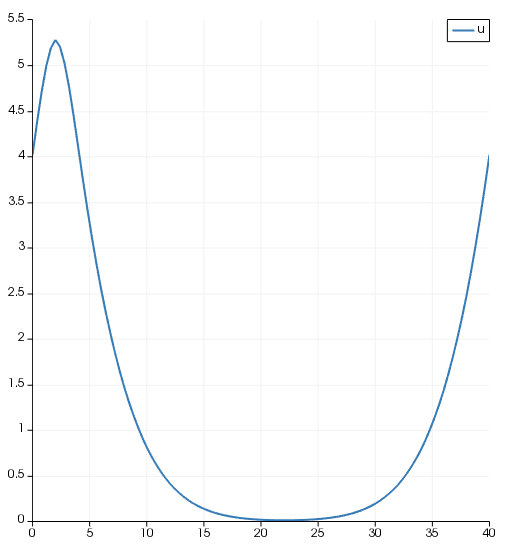
\includegraphics[width=\linewidth]{periodic_bc2_2}
			\caption{t=20.}
		\end{subfigure}
		\hfill
		\caption{Periodic BCs.}
		\label{fig:periodic}
	\end{figure}

	\subsection{advec2-t}

	\begin{itemize}
		\item \textit{advec2-t.i}
		\item 1D generated mesh with libmesh
		\item Uses DG Kernels
		\item TemperatureInflowBC and TemperatureOutflowBC
		\item Transient problem
	\end{itemize}

    Very similar to \textit{advec1-t.i}.
    Adds volumetric source.
    Figure \ref{fig:advec2-t} shows the results.
    It is correct. $\rho(L, t \rightarrow \infty) - \rho(0, t) = q/v*L = 200$

	\begin{equation}
    \frac{\partial}{\partial t}\rho + v \frac{\partial}{\partial x} \rho = \dot{q}
	\end{equation}

	\begin{itemize}
		\item IC: $\rho(x, 0) = 100 + 10 sin(\frac{\pi}{L} x)$
		\item BC: $\rho(0, t) = 100$
		\item $v = 0.5$
		\item $L = 100$
		\item $q = 1$
	\end{itemize}

	\begin{figure}[htbp!]
		\centering
		\begin{subfigure}[t]{0.4\textwidth}
			\centering
			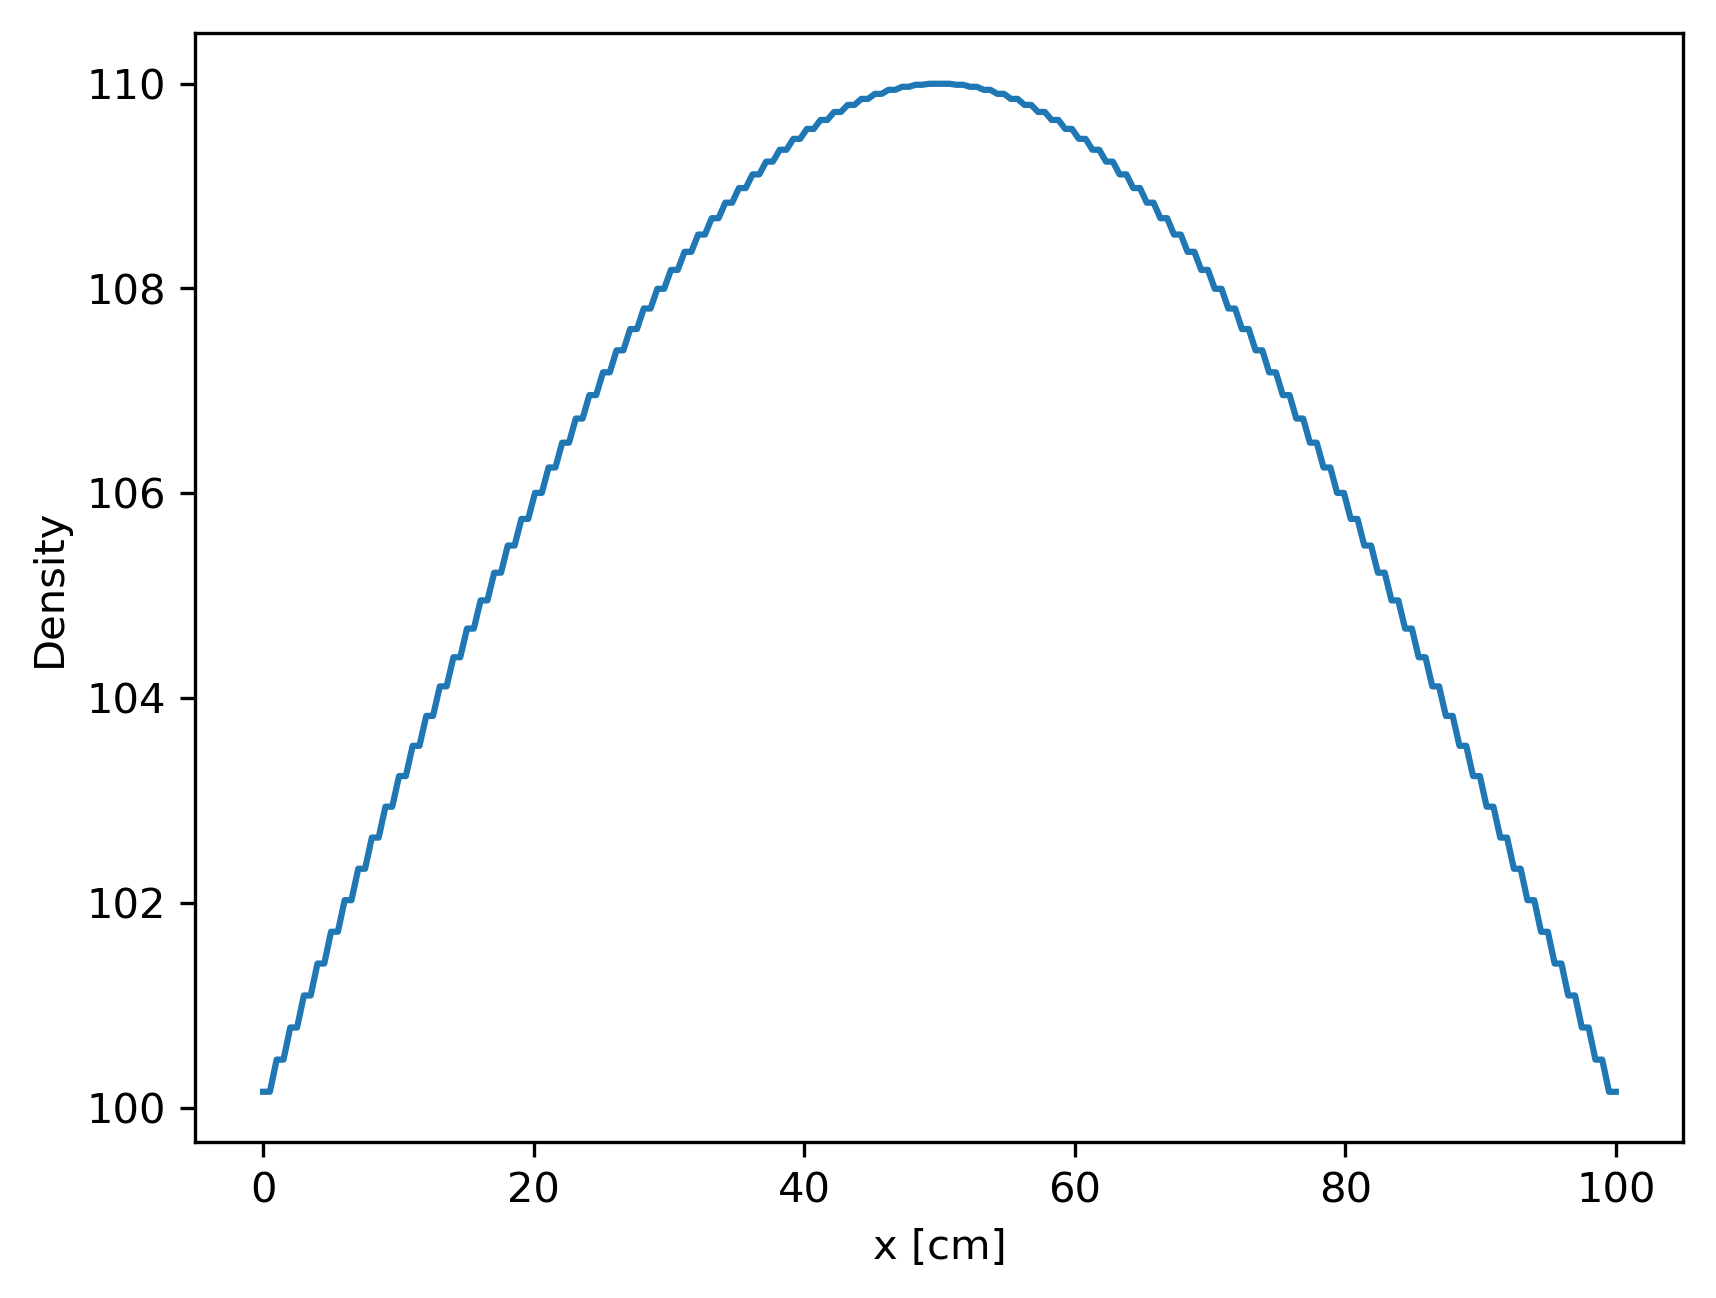
\includegraphics[width=\linewidth]{advec2-t-0}
			\caption{t=0.}
		\end{subfigure}
		\begin{subfigure}[t]{0.4\textwidth}
			\centering
			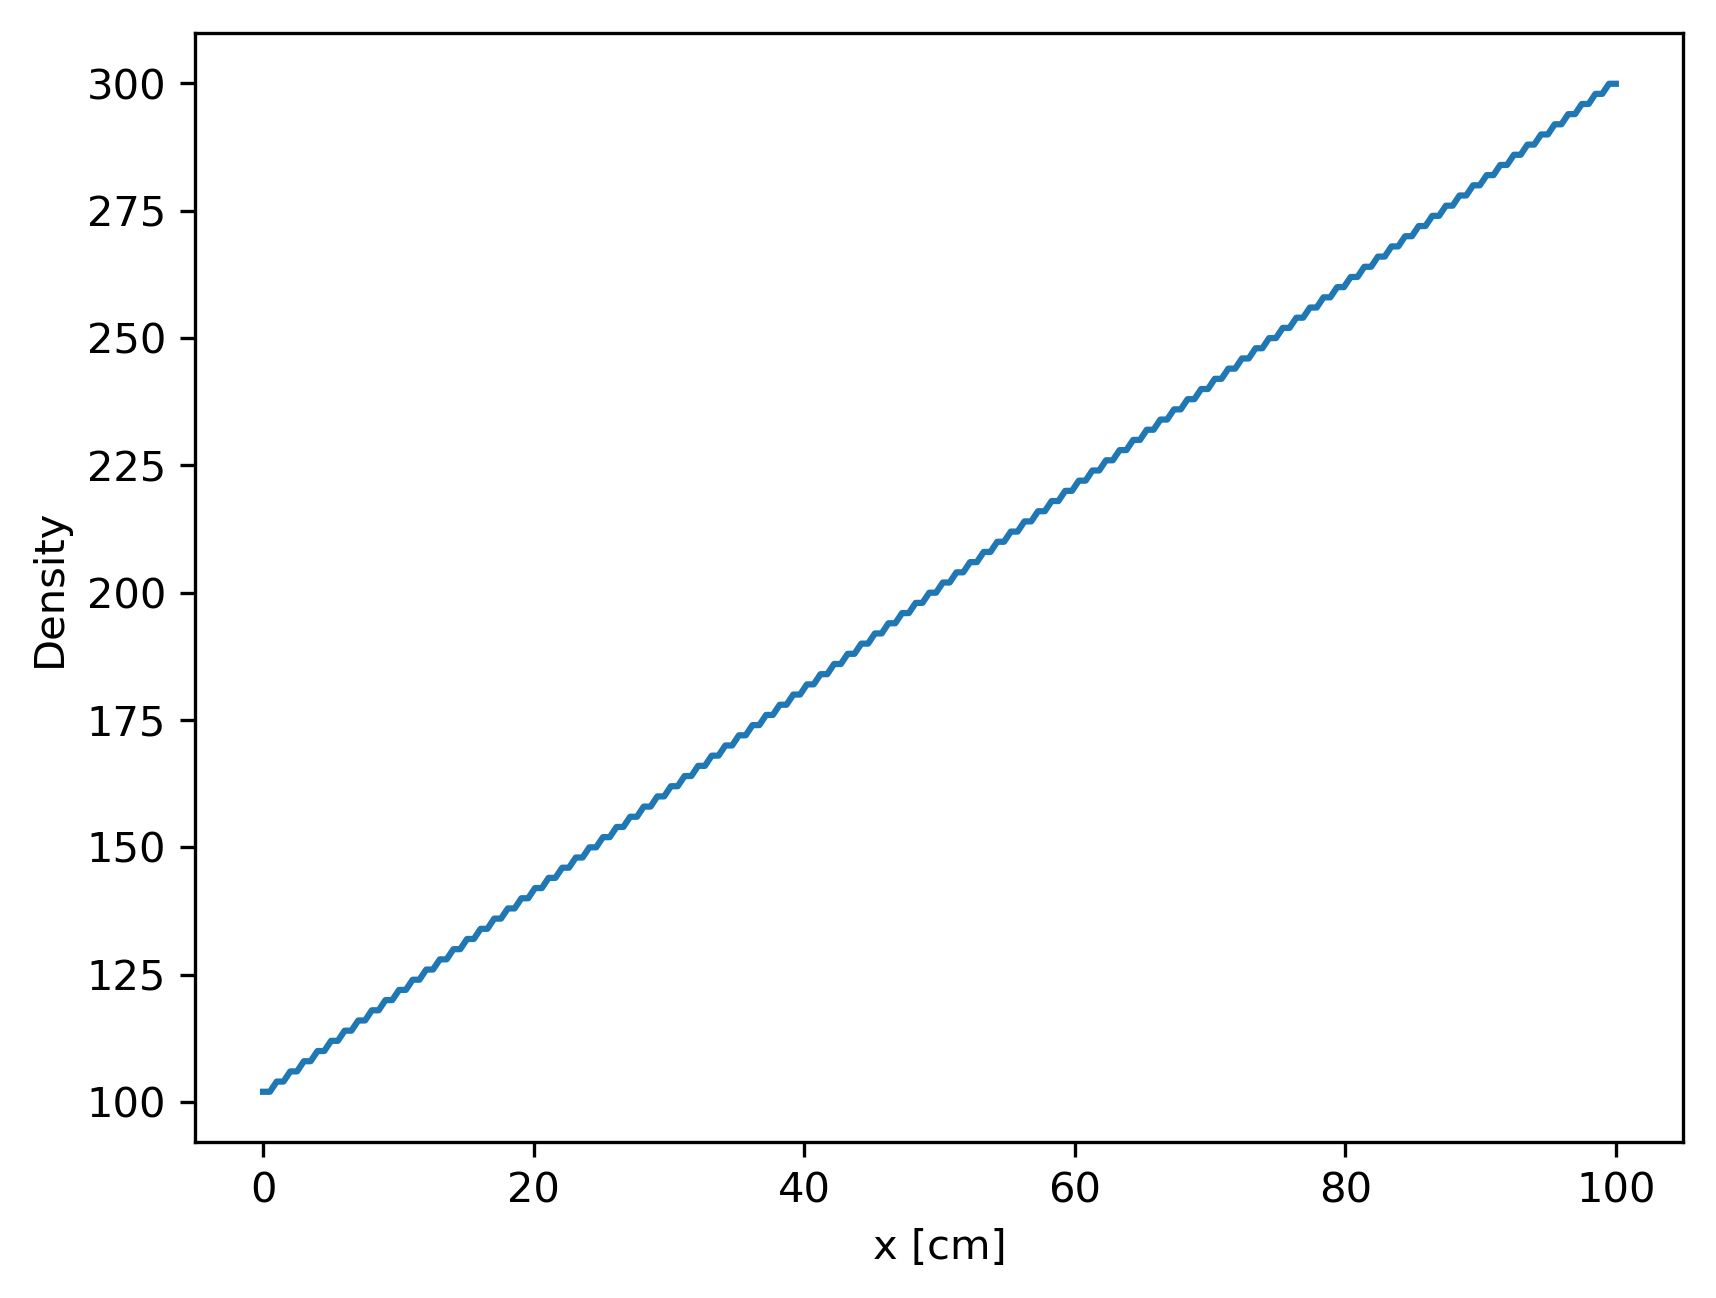
\includegraphics[width=\linewidth]{advec2-t-251}
			\caption{t=250.}
		\end{subfigure}
		\hfill
		\caption{Advected density with volumentric source.}
		\label{fig:advec2-t}
	\end{figure}

	\subsection{advec2-ss}

	\begin{itemize}
		\item \textit{advec2-ss.i}
		\item 1D generated mesh with libmesh
		\item Uses DG Kernels
		\item Inflow and OutflowBC
		\item Steady problem
	\end{itemize}

    Same as \textit{advec2-t} but steady state.
    Figure \ref{fig:advec2-ss} shows the results.
    It is correct. $\rho(L) - \rho(0) = q/v*L = 200$

	\begin{equation}
    v \frac{\partial}{\partial x} \rho = \dot{q}
	\end{equation}

	\begin{itemize}
		\item BC: $\rho(0, t) = 100$
		\item $v = 0.5$
		\item $L = 100$
		\item $q = 1$
	\end{itemize}

	\begin{figure}[htbp!]
		\centering
		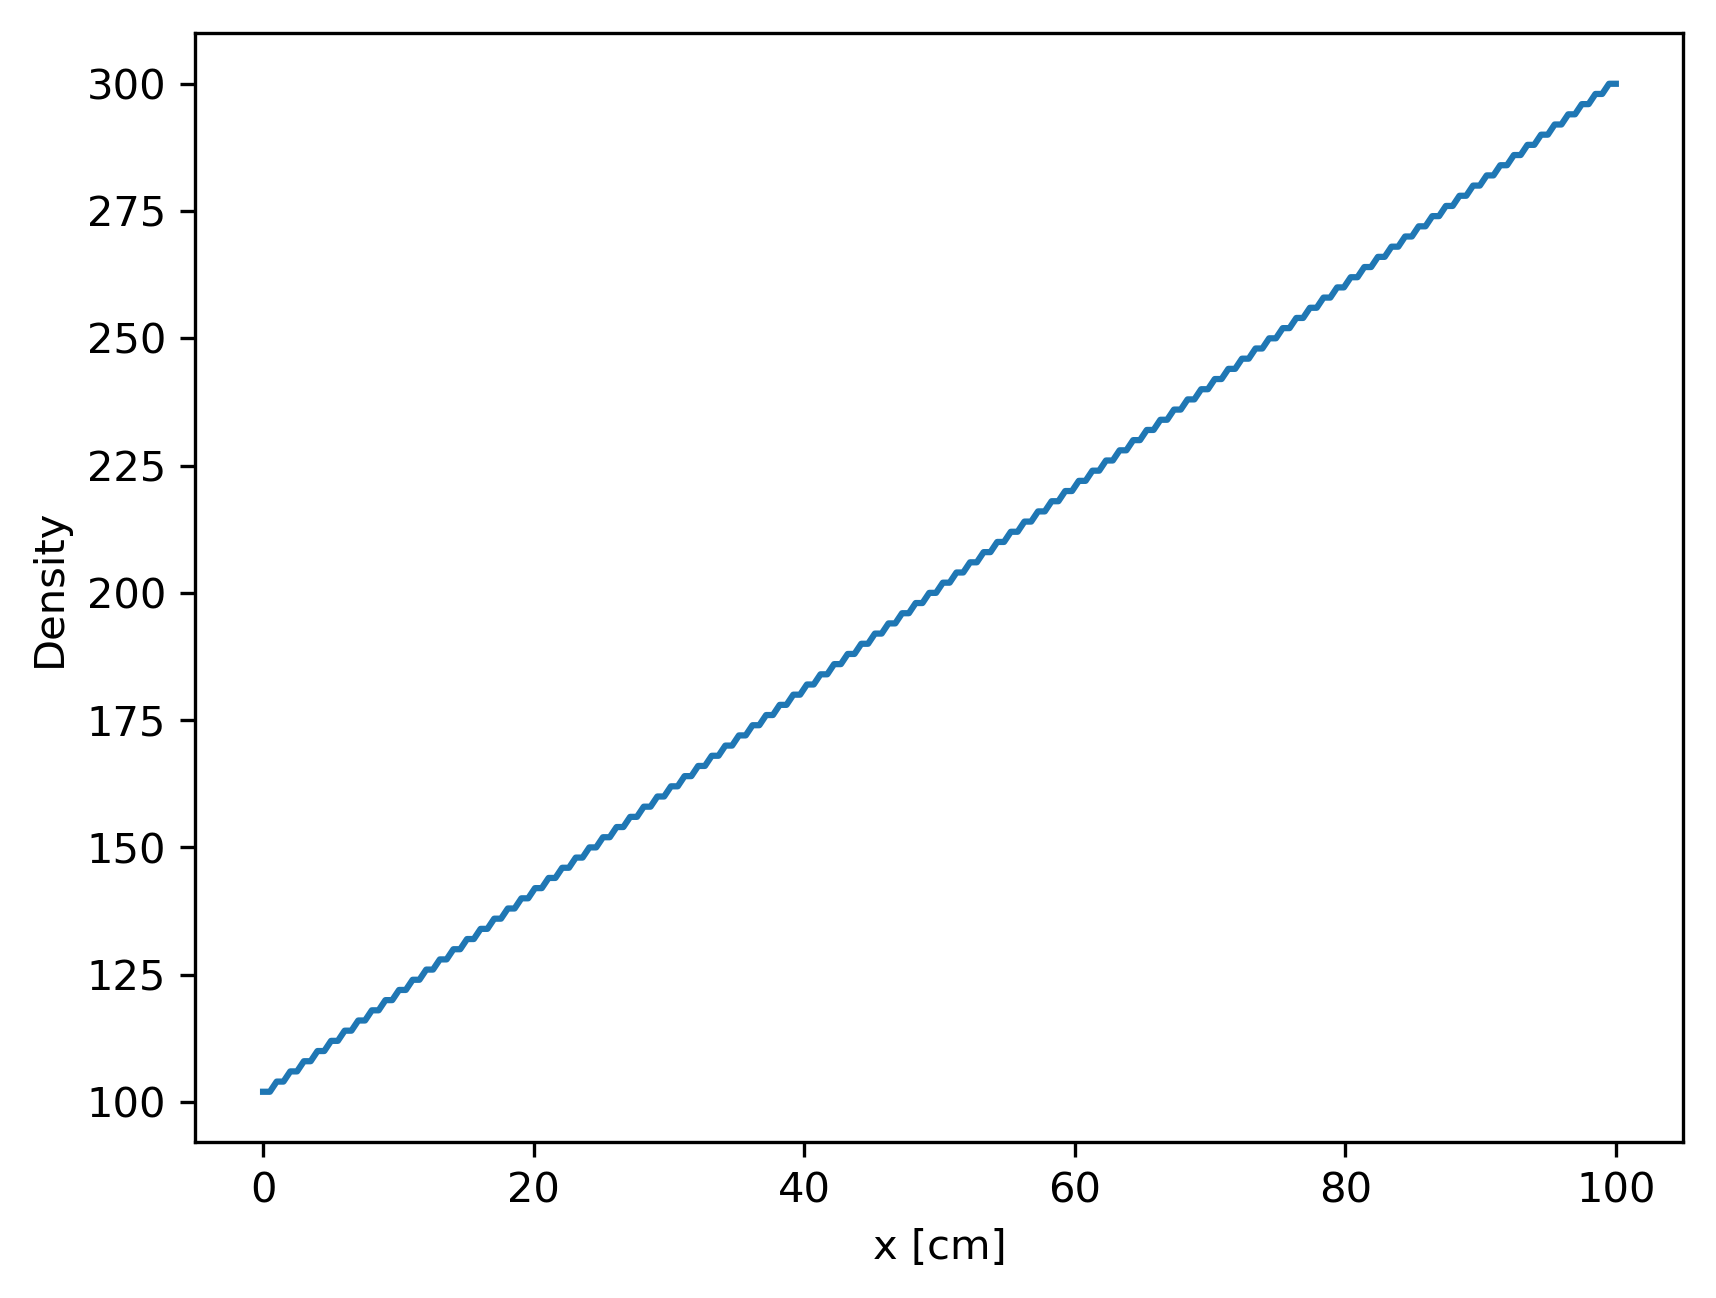
\includegraphics[height=5cm]{advec2-ss}
		\caption{Steady state solution.}
		\label{fig:advec2-ss}
	\end{figure}

	\subsection{advec3-t}

	\begin{itemize}
		\item \textit{advec3-t.i}
		\item 1D generated mesh with libmesh
		\item Uses DG Kernels
		\item TemperatureInflowBC and TemperatureOutflowBC
		\item Transient problem
	\end{itemize}

    Very similar to \textit{advec1-t.i}. Solves for the temperature advection equation.
    Advects BC.
    Figure \ref{fig:advec3-t} shows the results.

	\begin{equation}
    \rho c_p \frac{\partial}{\partial t}T + \rho c_p v \frac{\partial}{\partial x} T = 0
	\end{equation}

	\begin{itemize}
		\item BC: $T(0, t) = 930$
		\item IC: $T(x, 0) = 930$
		\item $\rho = 1e-2$
		\item $c_p = 2e3$
		\item $v = 0.5$
		\item $L = 100$
	\end{itemize}

	\begin{figure}[htbp!]
		\centering
		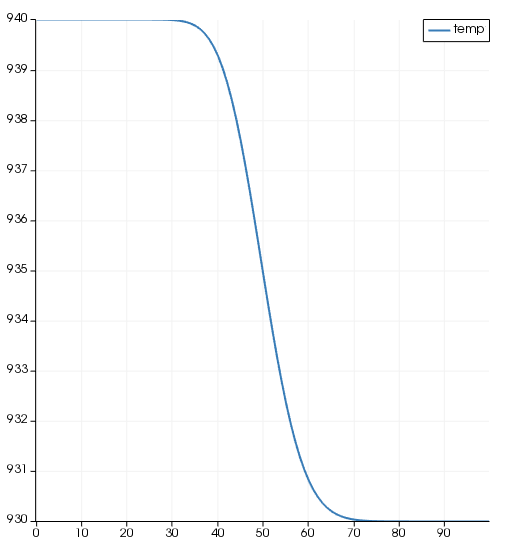
\includegraphics[height=5cm]{advec3-t}
		\caption{Advects BC.}
		\label{fig:advec3-t}
	\end{figure}

	\subsection{advec4-t}

	\begin{itemize}
		\item \textit{advec4-t.i}
		\item 1D generated mesh with libmesh
		\item Uses DG Kernels
		\item TemperatureInflowBC and TemperatureOutflowBC
		\item Transient problem
	\end{itemize}

    Similar to \textit{advec4-t.i}
    Adds a point source and solves for temperature.
    Figure \ref{fig:advec4-t} shows the results.
    It is correct. $T(L) - T(0) = q/(\rho c_p v )*L = 10$

	\begin{equation}
    \rho c_p \frac{\partial}{\partial t}T + \rho c_p v \frac{\partial}{\partial x} T = \dot{q}
	\end{equation}

	\begin{itemize}
		\item BC: $T(0, t) = 930$
		\item IC: $T(x, 0) = 930$
		\item $\rho = 1e-2$
		\item $c_p = 2e3$
		\item $v = 0.5$
		\item $L = 100$
		\item $q = 1$
	\end{itemize}

	\begin{figure}[htbp!]
		\centering
		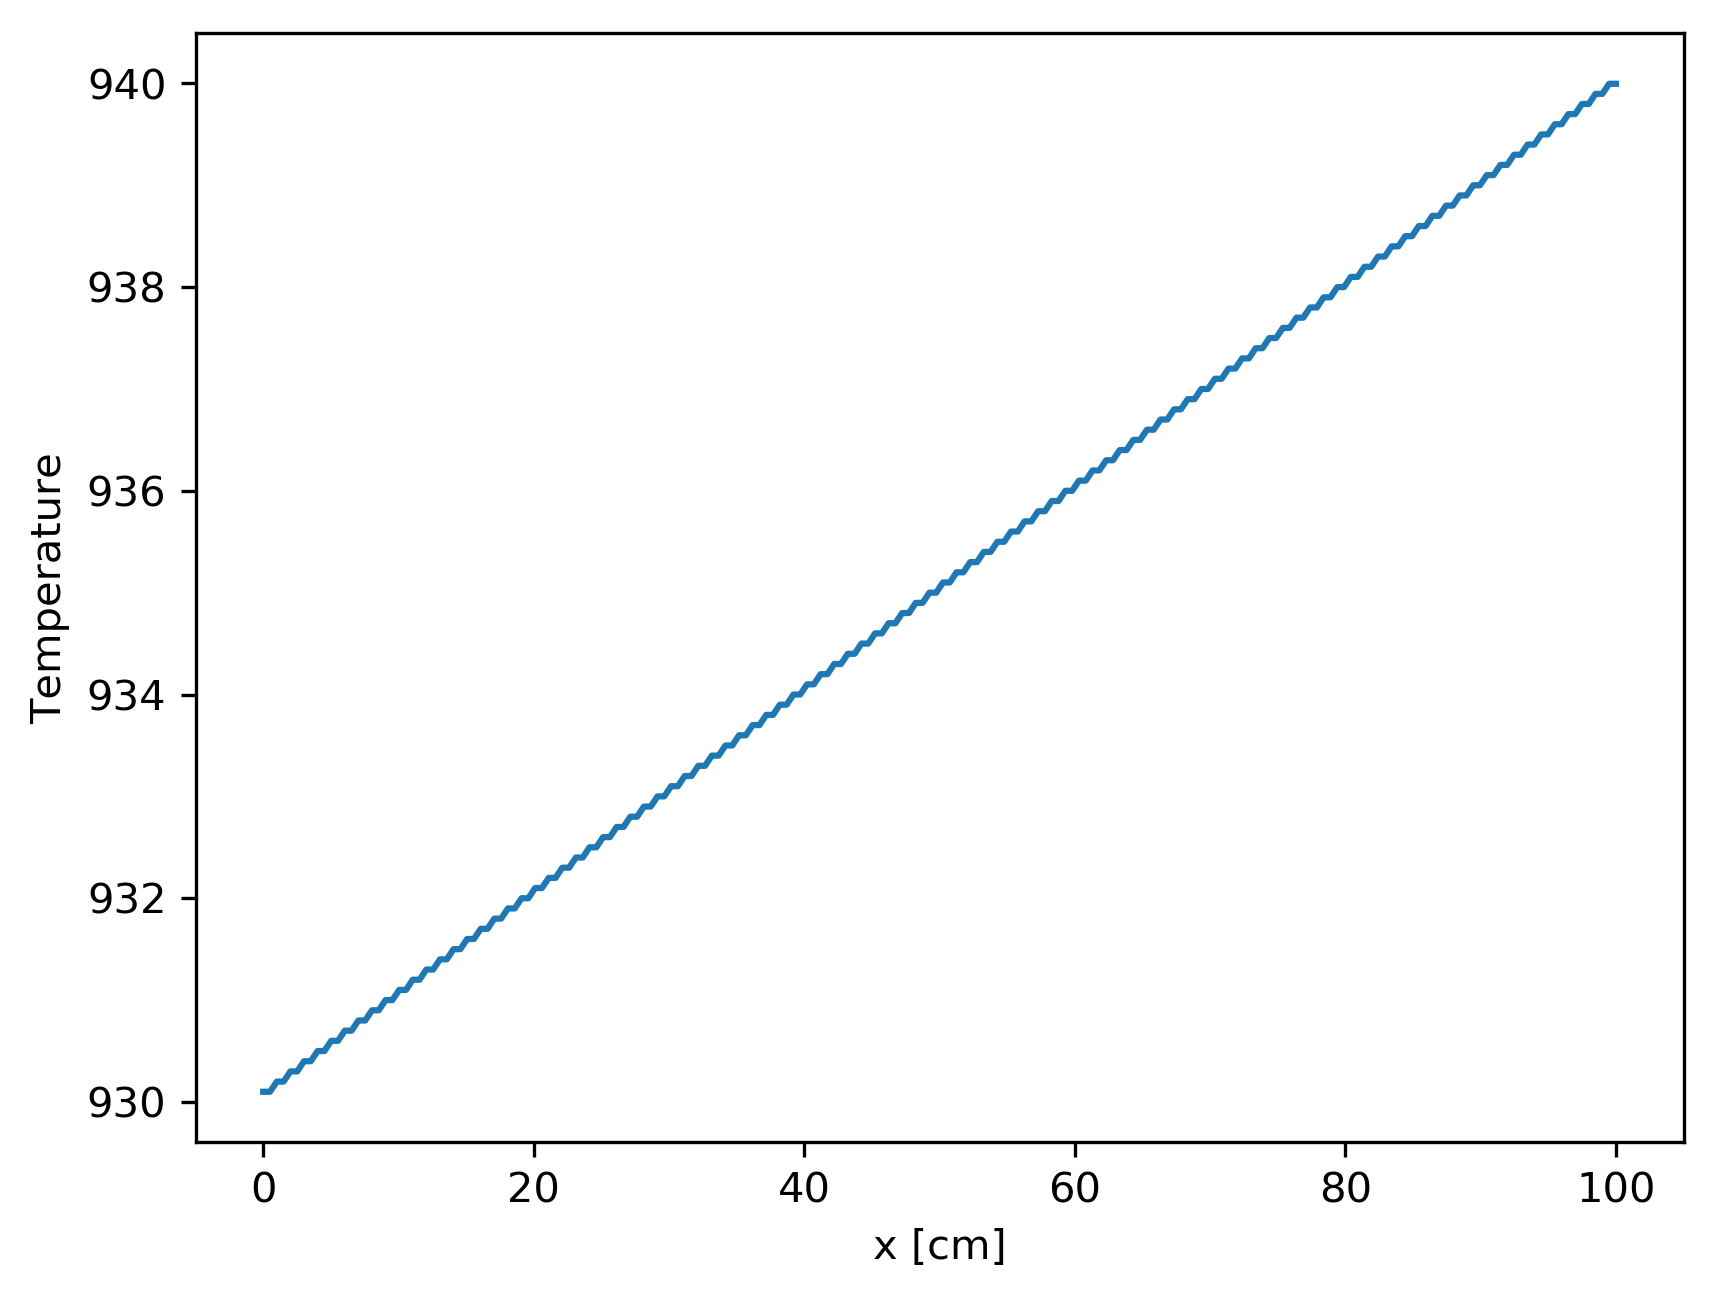
\includegraphics[height=5cm]{advec4-t-251}
		\caption{t=250.}
		\label{fig:advec4-t}
	\end{figure}

	\subsection{advec5-t}

	\begin{itemize}
		\item \textit{advec5-t.i}
		\item pseudo-1D: GeneratedMesh
		\item Uses DG Kernels
		\item TemperatureInflowBC and TemperatureOutflowBC
		\item Transient problem
	\end{itemize}

    Similar to \textit{advec4-t.i} but has a $q''$ on the wall.
    Figure \ref{fig:advec5-t} shows the results.

	\begin{equation}
    \rho c_p \frac{\partial}{\partial t}T + \rho c_p v \frac{\partial}{\partial x} T = 0
	\end{equation}

    This is not the real equation. When using the Galerkin method, a new term appears due to the neumann BC.

	\begin{itemize}
		\item IC: $T(x, y, 0) = 930$
		\item BC: $T(x, 0, t) = 930$
		\item BC: $q''(0, y, t) = 10 sin (\pi/L y)$
		\item $\rho = 1e-2$
		\item $c_p = 2e3$
		\item $v = 0.5$
		\item $L = 100$
		\item $\Delta_x = 2$
	\end{itemize}

	\begin{equation}
	T(L) - T(0) = \frac{1}{\rho c_p v}\frac{1}{\Delta_x}\int^L_0 q'' dx = \frac{1}{10} \frac{1}{2} \frac{10 \times 2 \times L}{\pi}
	\end{equation}

	\begin{figure}[htbp!]
		\centering
		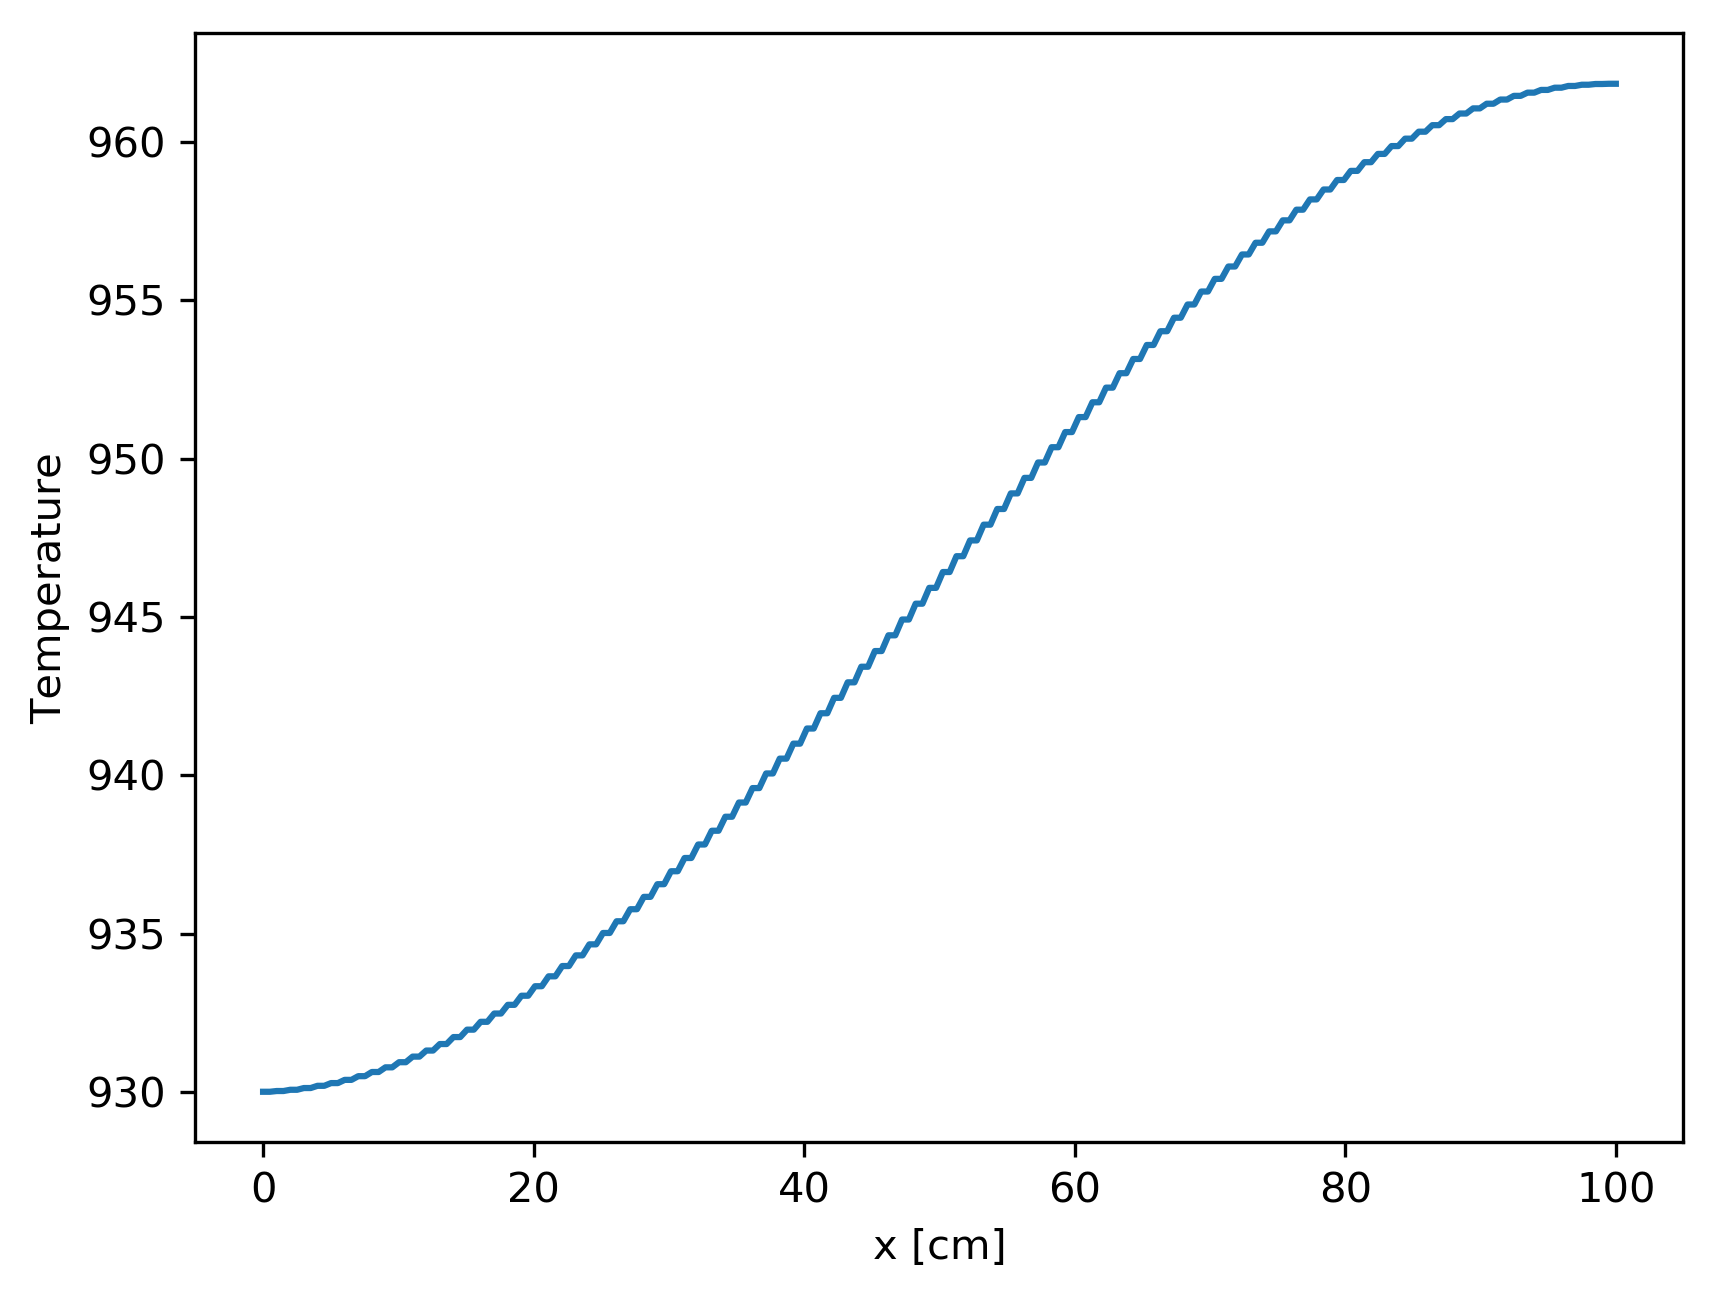
\includegraphics[height=5cm]{advec5-t-251}
		\caption{Advects temperature while wall is been heated.}
		\label{fig:advec5-t}
	\end{figure}

	\subsection{advec5-ss}

	\begin{itemize}
		\item \textit{advec5-ss.i}
		\item pseudo-1D: GeneratedMesh
		\item Uses DG Kernels
		\item TemperatureInflowBC and TemperatureOutflowBC
		\item Steady state problem
	\end{itemize}

    Steady state version of \textit{advec5-t.i}.
    Figure \ref{fig:advec5-ss} shows the results.

	\begin{equation}
    \rho c_p v \frac{\partial}{\partial x} T = 0
	\end{equation}

	This is not the real equation. When using the Galerkin method, a new term appears due to the neumann BC.

	\begin{itemize}
		\item BC: $T(x, 0) = 930$
		\item BC: $q''(0, y) = 10 sin (\pi/L y)$
		\item $\rho = 1e-2$
		\item $c_p = 2e3$
		\item $v = 0.5$
		\item $L = 100$
		\item $\Delta_x = 2$
	\end{itemize}

	\begin{equation}
	T(L) - T(0) = \frac{1}{\rho c_p v}\frac{1}{\Delta_x}\int^L_0 q'' dx = \frac{1}{10} \frac{1}{2} \frac{10 \times 2 \times L}{\pi}
	\end{equation}

	\begin{figure}[htbp!]
		\centering
		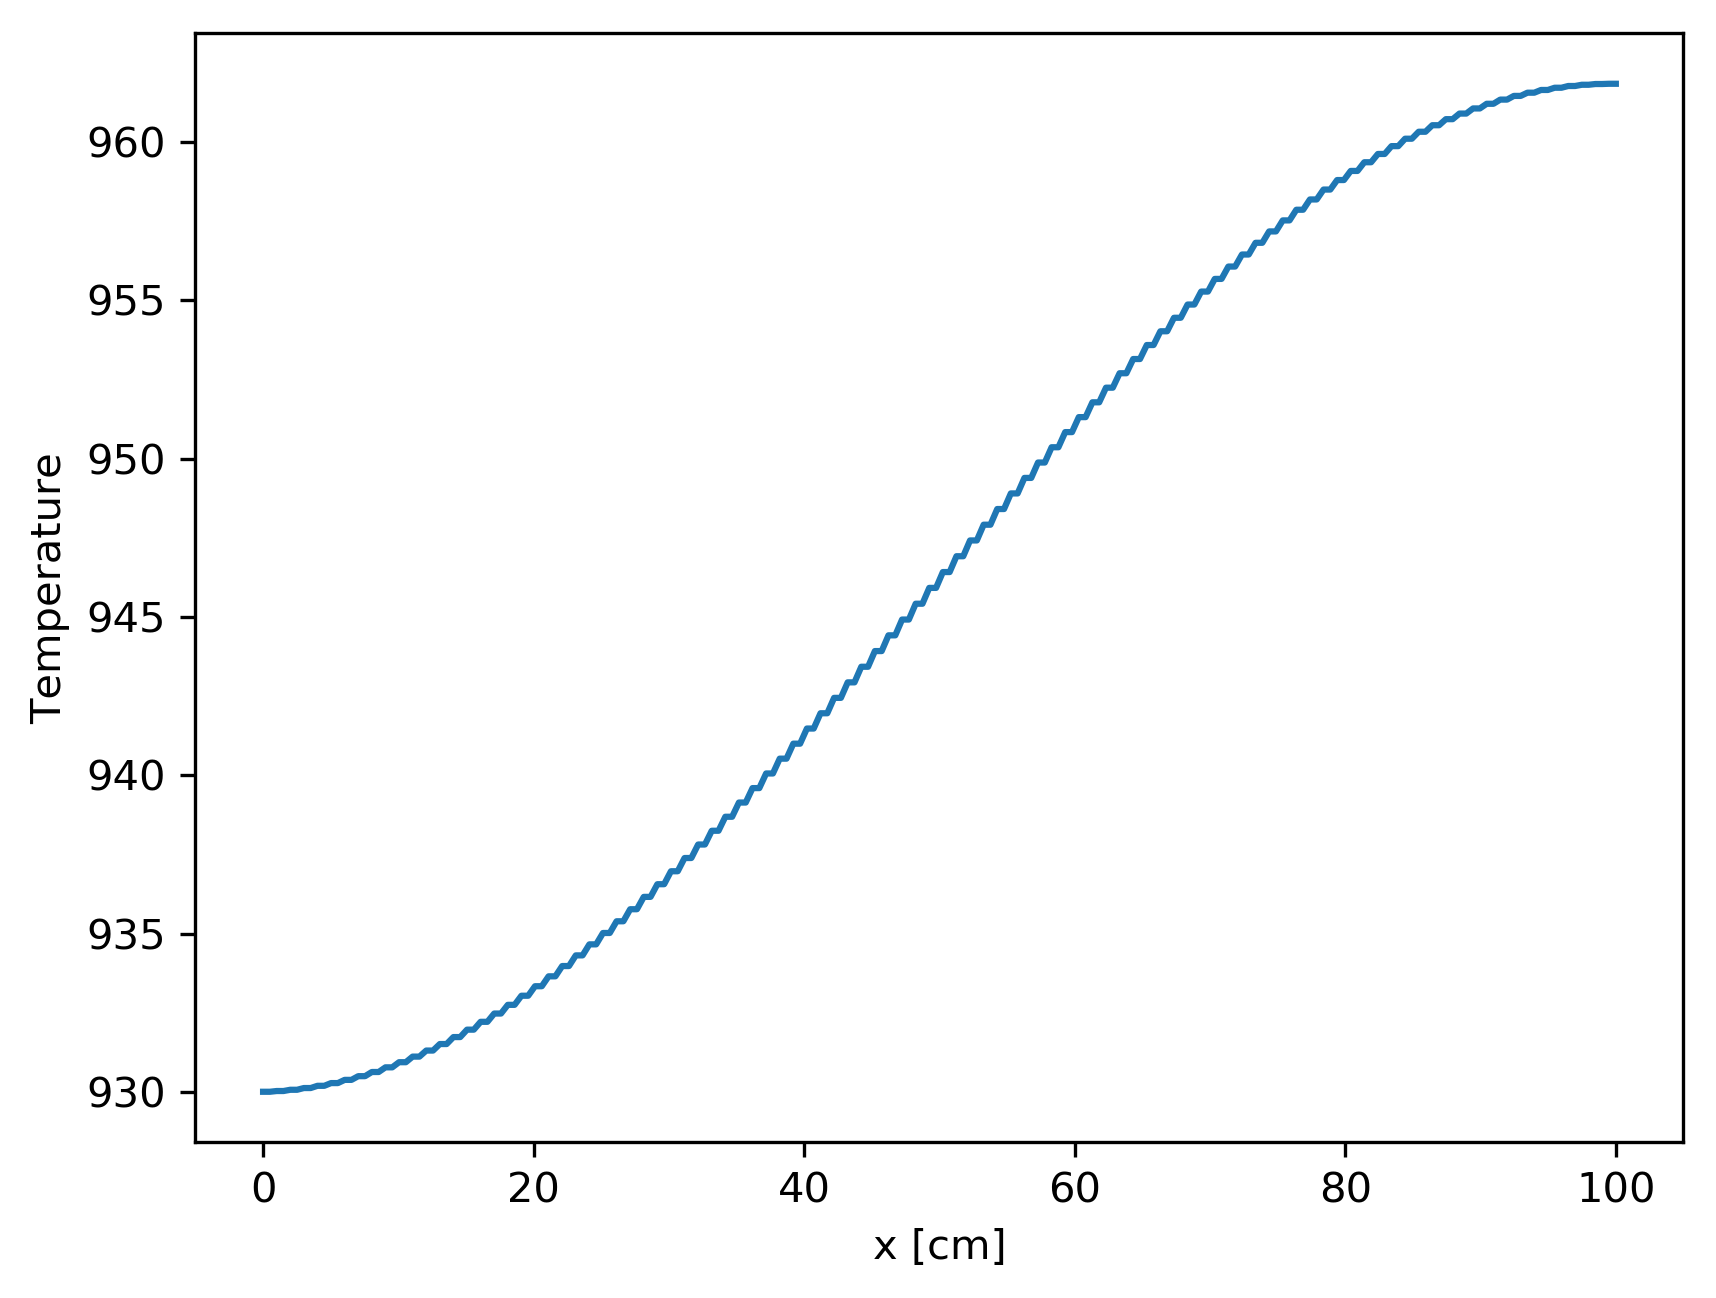
\includegraphics[height=5cm]{advec5-ss}
		\caption{Advects temperature while wall is been heated.}
		\label{fig:advec5-ss}
	\end{figure}

\pagebreak
\bibliographystyle{plain}
% \bibliography{bibliography}

\end{document}

	% \begin{figure}[htbp!]
	% 	\centering
	% 	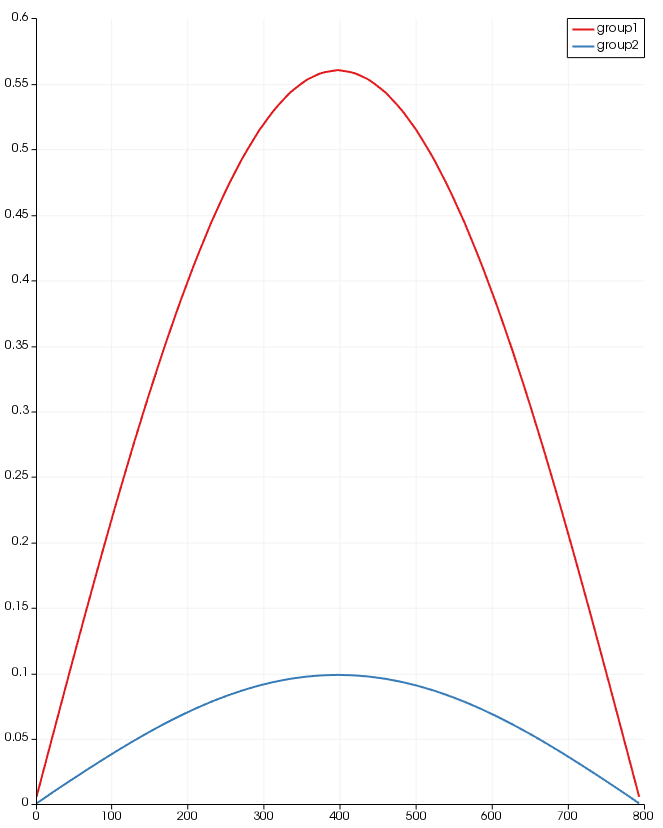
\includegraphics[height=5cm]{1D-fuel-eig}
	% 	\caption{Steady state Group 1 and 2 fluxes.}
	% 	\label{fig:1D-fuel-eig}
	% \end{figure}